\section{Presentation Logic Layer}

%What pages will be present in your project? briefly indicate how your web site will be organized

The web application is divided in the following pages:
\begin{itemize}
	\item Homepage: This page contains the main information regarding the gym such as the available courses held in a given period, instructors, rooms, timetables, prices...
	\item The gym: This page contains information about the rooms of the gym.
	\item Courses : This page shows a list of the available courses with a brief description of them .
	\item Calendar : This page provides information about the lectures that are held in a given week. It shows the time, room and instructor for each lecture.
	\item Prices : This page shows the prices of each type of subscription for each course.
	\item Staff : This page provides general information about the staff (trainers and secretaries)
	\item Contact Us : This page contains the main information regarding the gym such as the e-mail address, the telephone number and the address.
	\item Login : This is a portal in which a guest user can login by providing his/her own credentials. After a successful login, it's possible to enter the personal area which is different based on the role of the user in the gym
	\item Register : This page provides a form that allows a guest user to register by providing his/her own personal information such as a valid e-mail address, Tax-Code, password... After a successful registration an e-mail will be sent to confirm the registration and the user must open the link written in the e-mail to be able to login to his/her account.
	\item Trainee : This is the personal area in which a user logged-in as a trainee can manage his/her personal info and book a lecture for a course for which he/she is subscribed. The trainer can also mark the presence of trainees during his/her lecture and add other attending trainee that have not booked that lecture if there are available spots left.
	\item Trainer: This  is the personal area, accessible only by trainers, containing information about the courses held by the logged-in trainer and his upcoming lectures.
	\item Secretary : This is the personal area accessible only by a user logged-in as secretary. Here it is possible to add/cancel/postpone lectures, add a substitutive trainer for a lecture, add a subscription for a user, add a medical certificate for a user, create other accounts.
\end{itemize}

\newpage
\subsection{Mockups}

\subsubsection{Home Page}
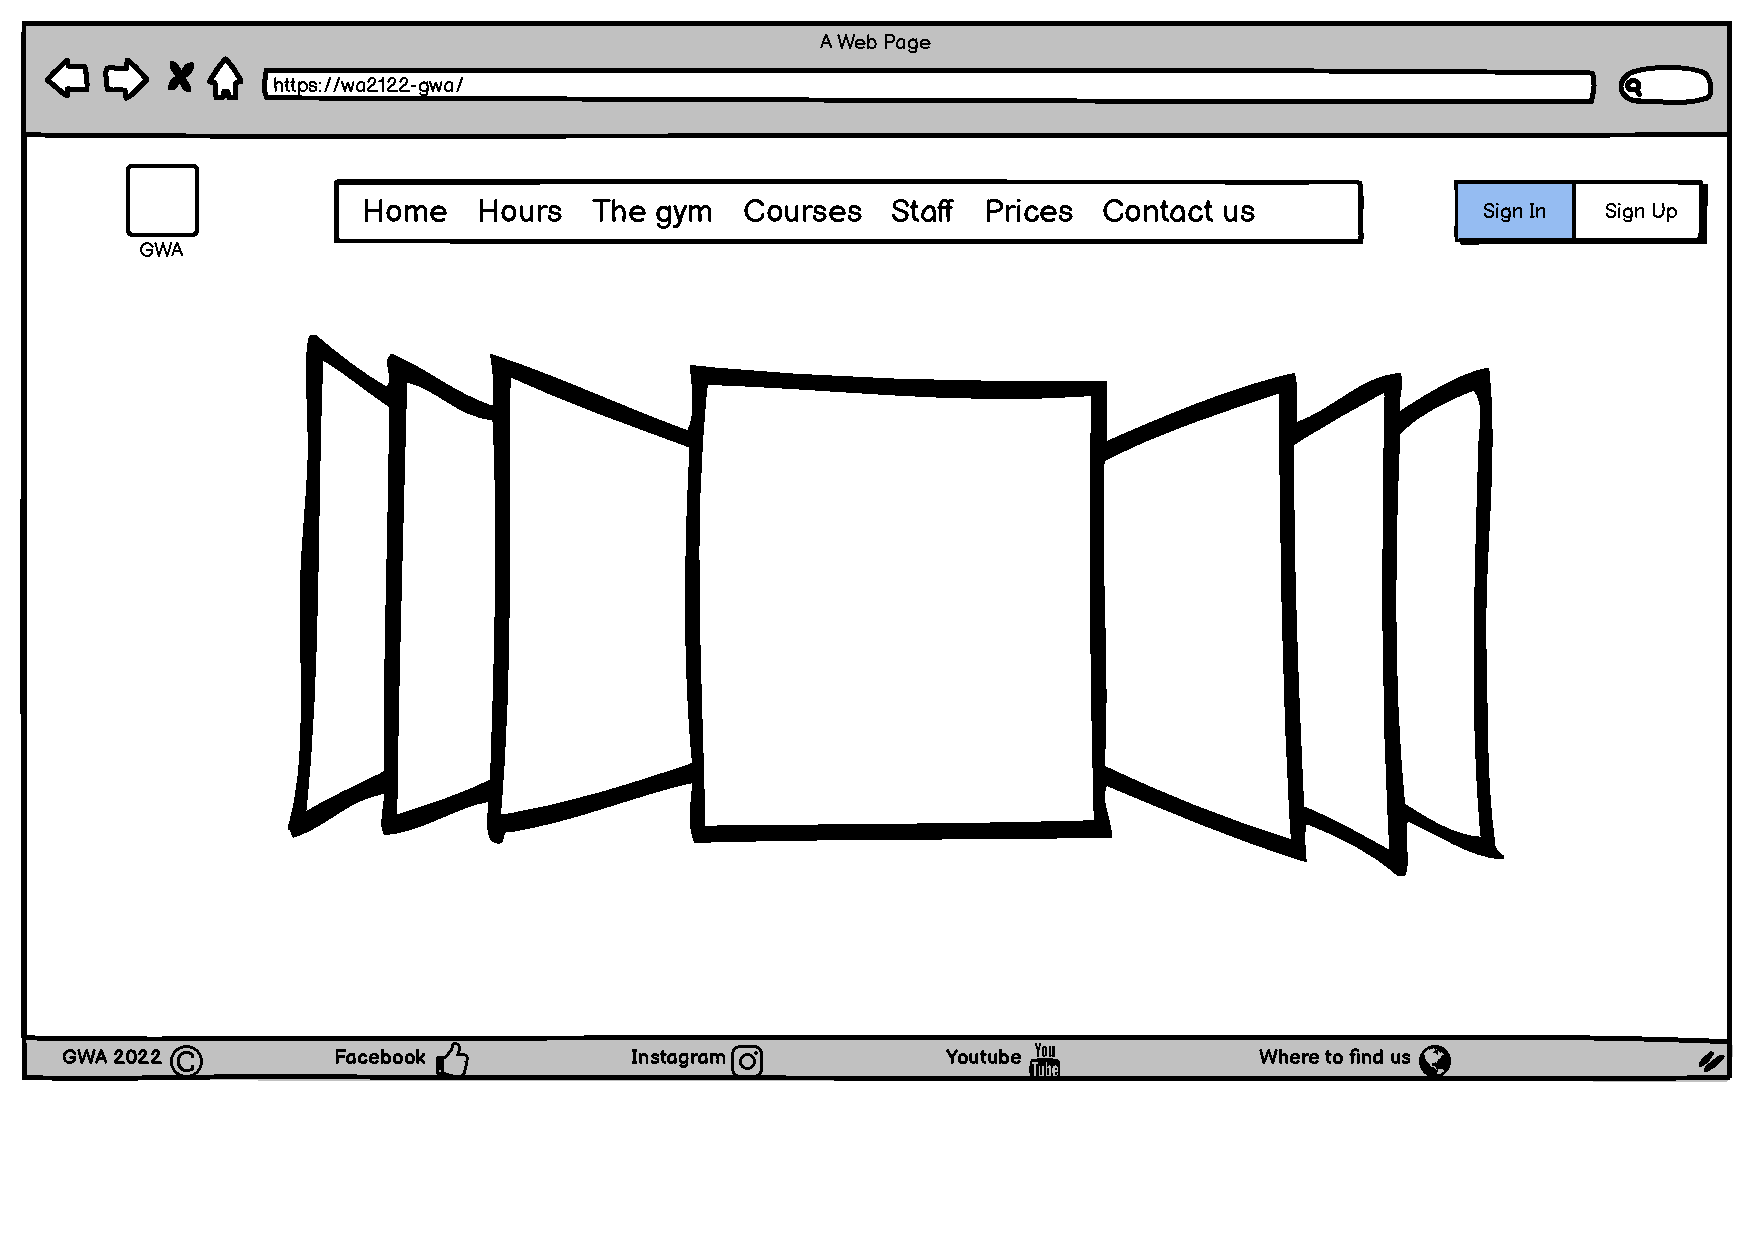
\includegraphics[width=\columnwidth]{InterfaceMockup/Index.pdf}

\subsubsection{The Gym}
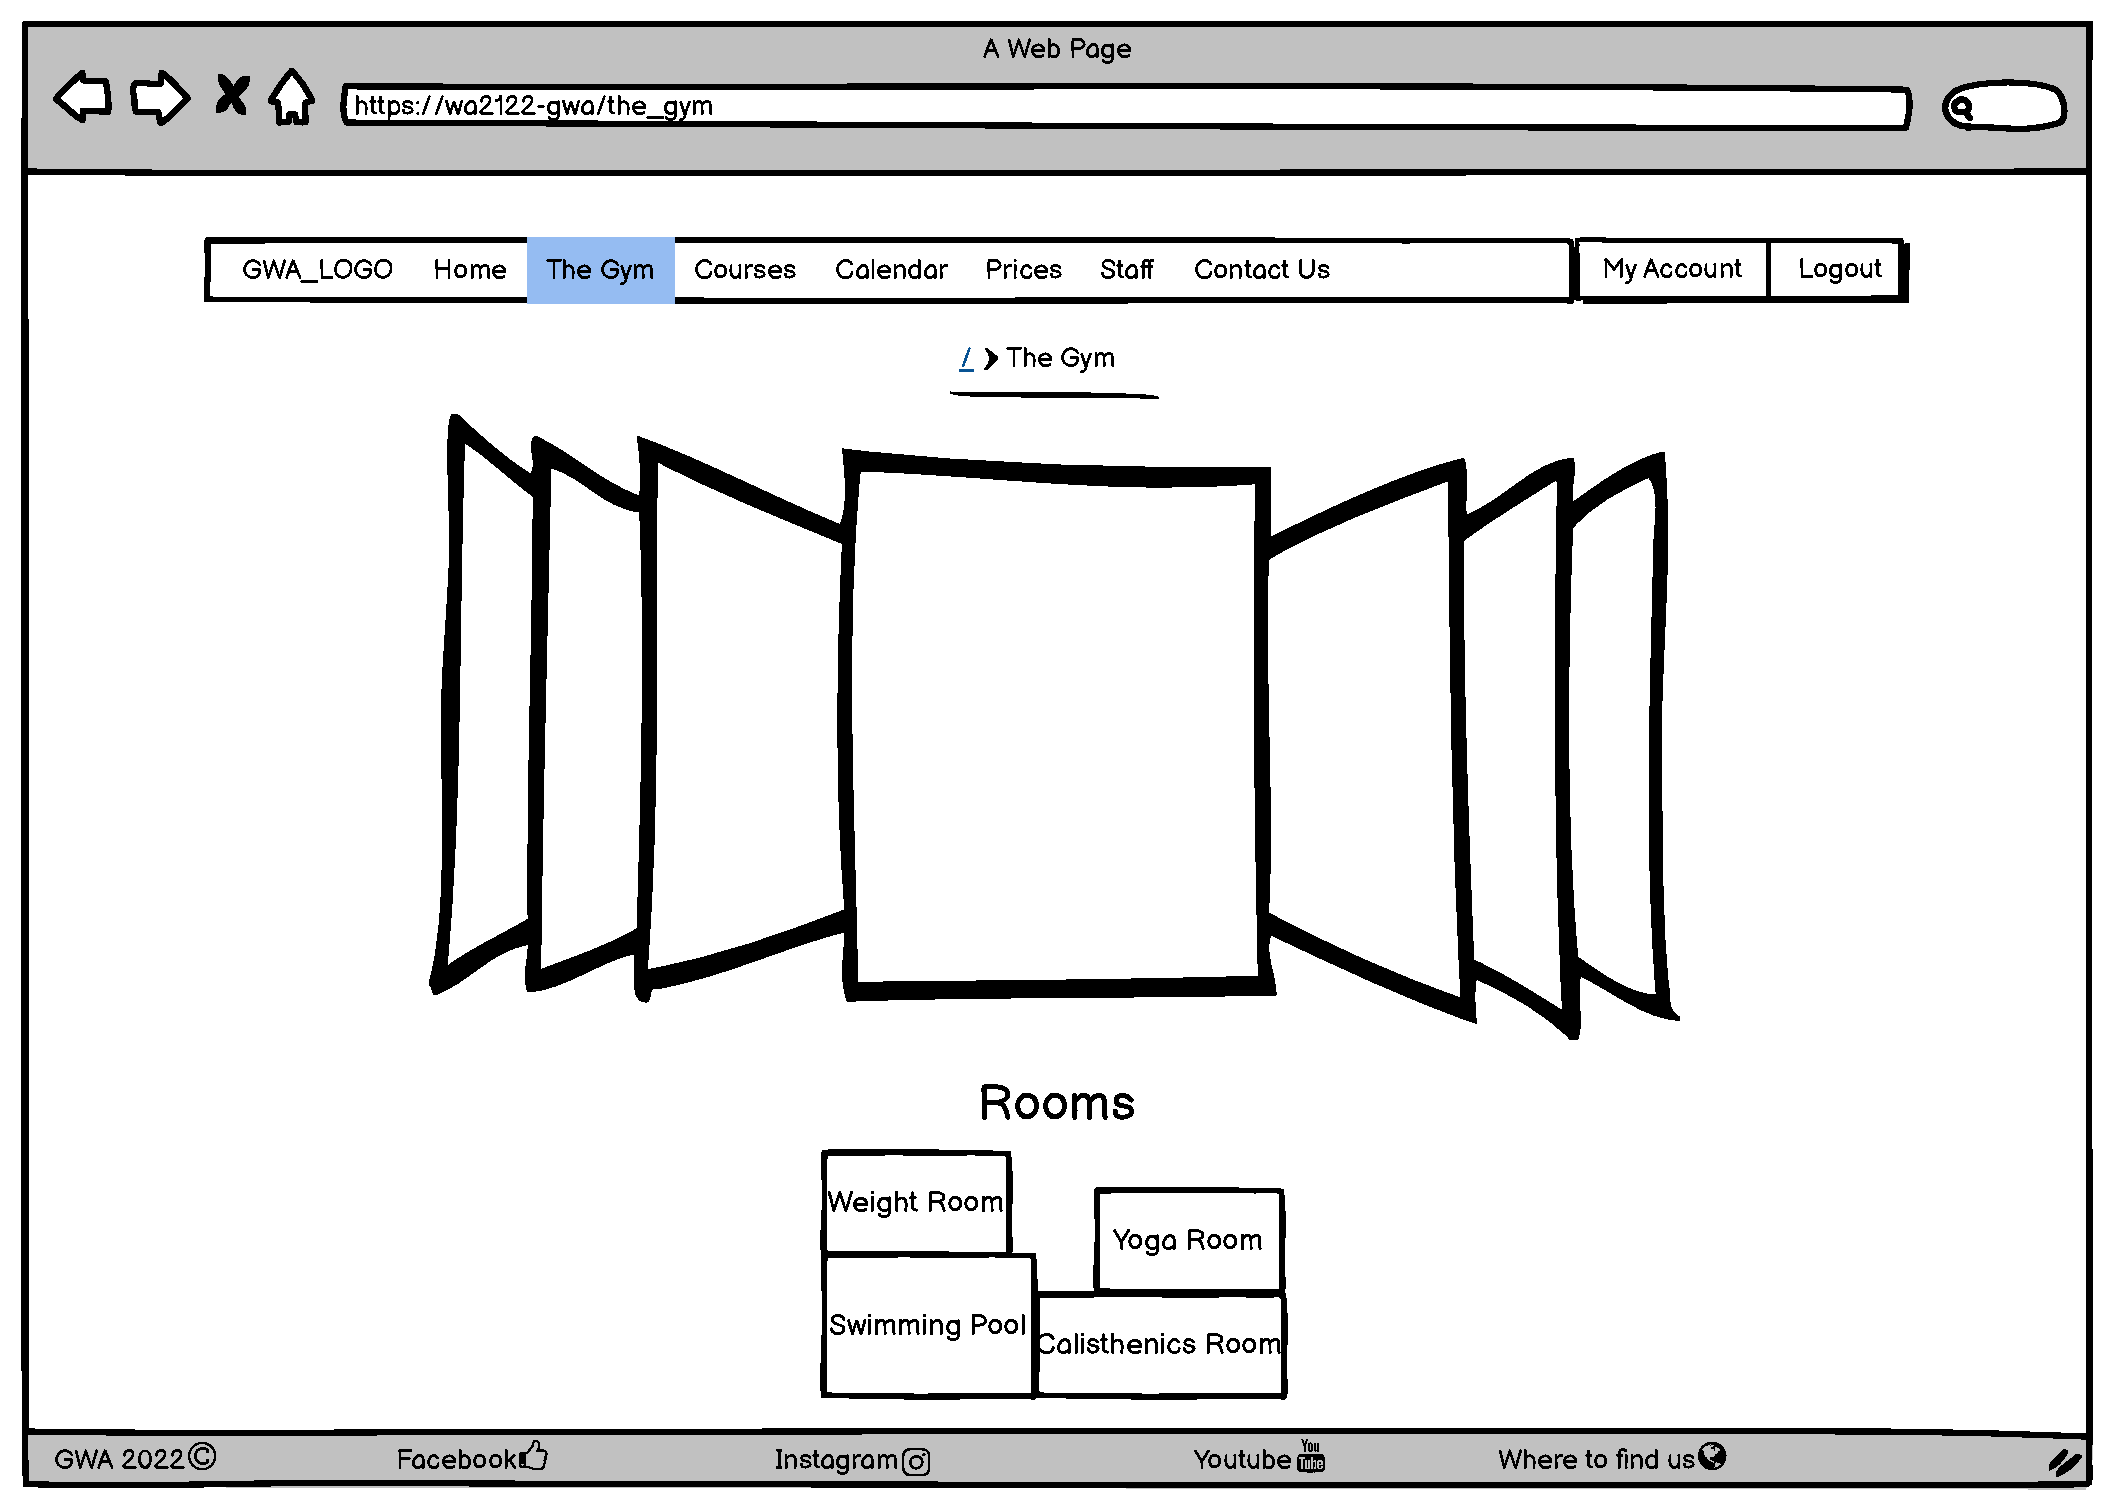
\includegraphics[width=\columnwidth]{InterfaceMockup/TheGym/TheGym_desktopVersion.pdf}

\subsubsection{Calendar}
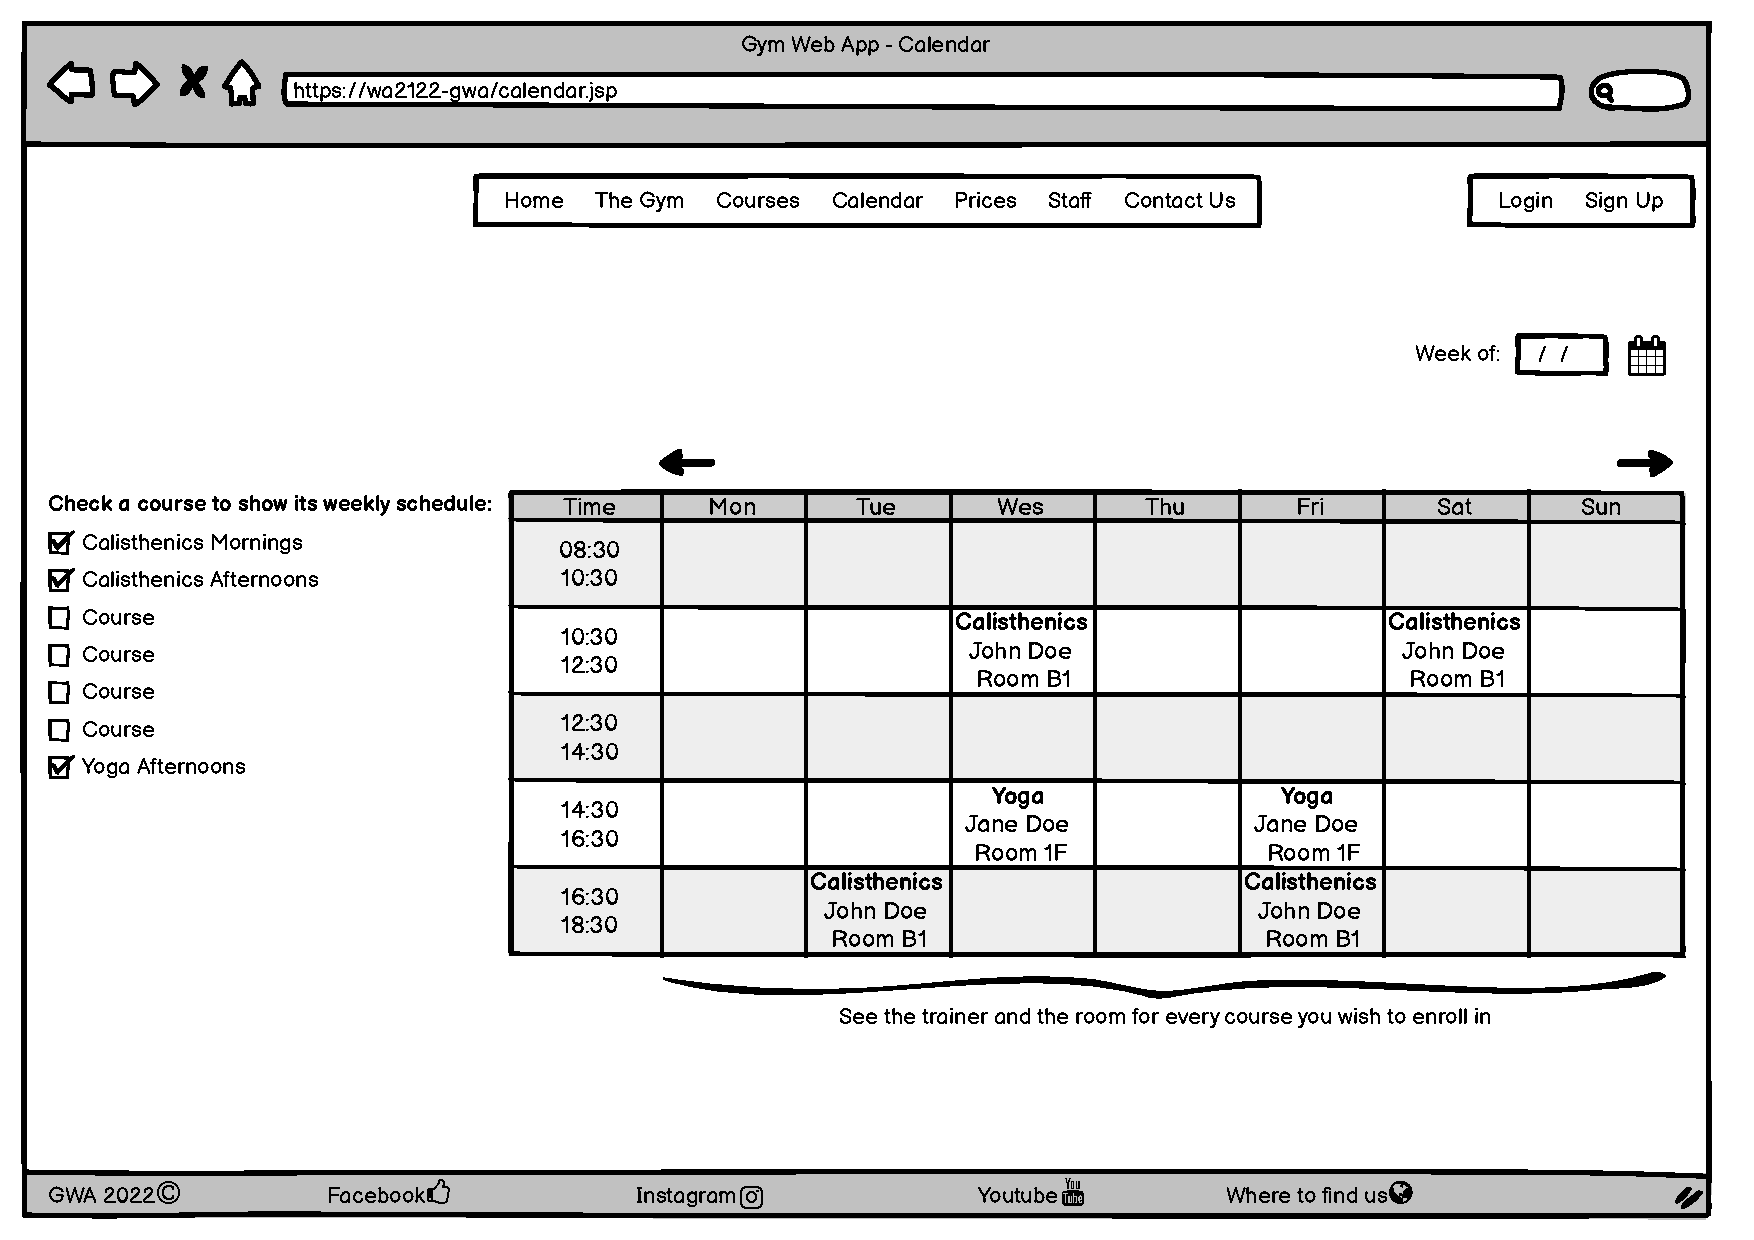
\includegraphics[width=\columnwidth]{InterfaceMockup/Calendar.pdf}

\subsubsection{Prices}
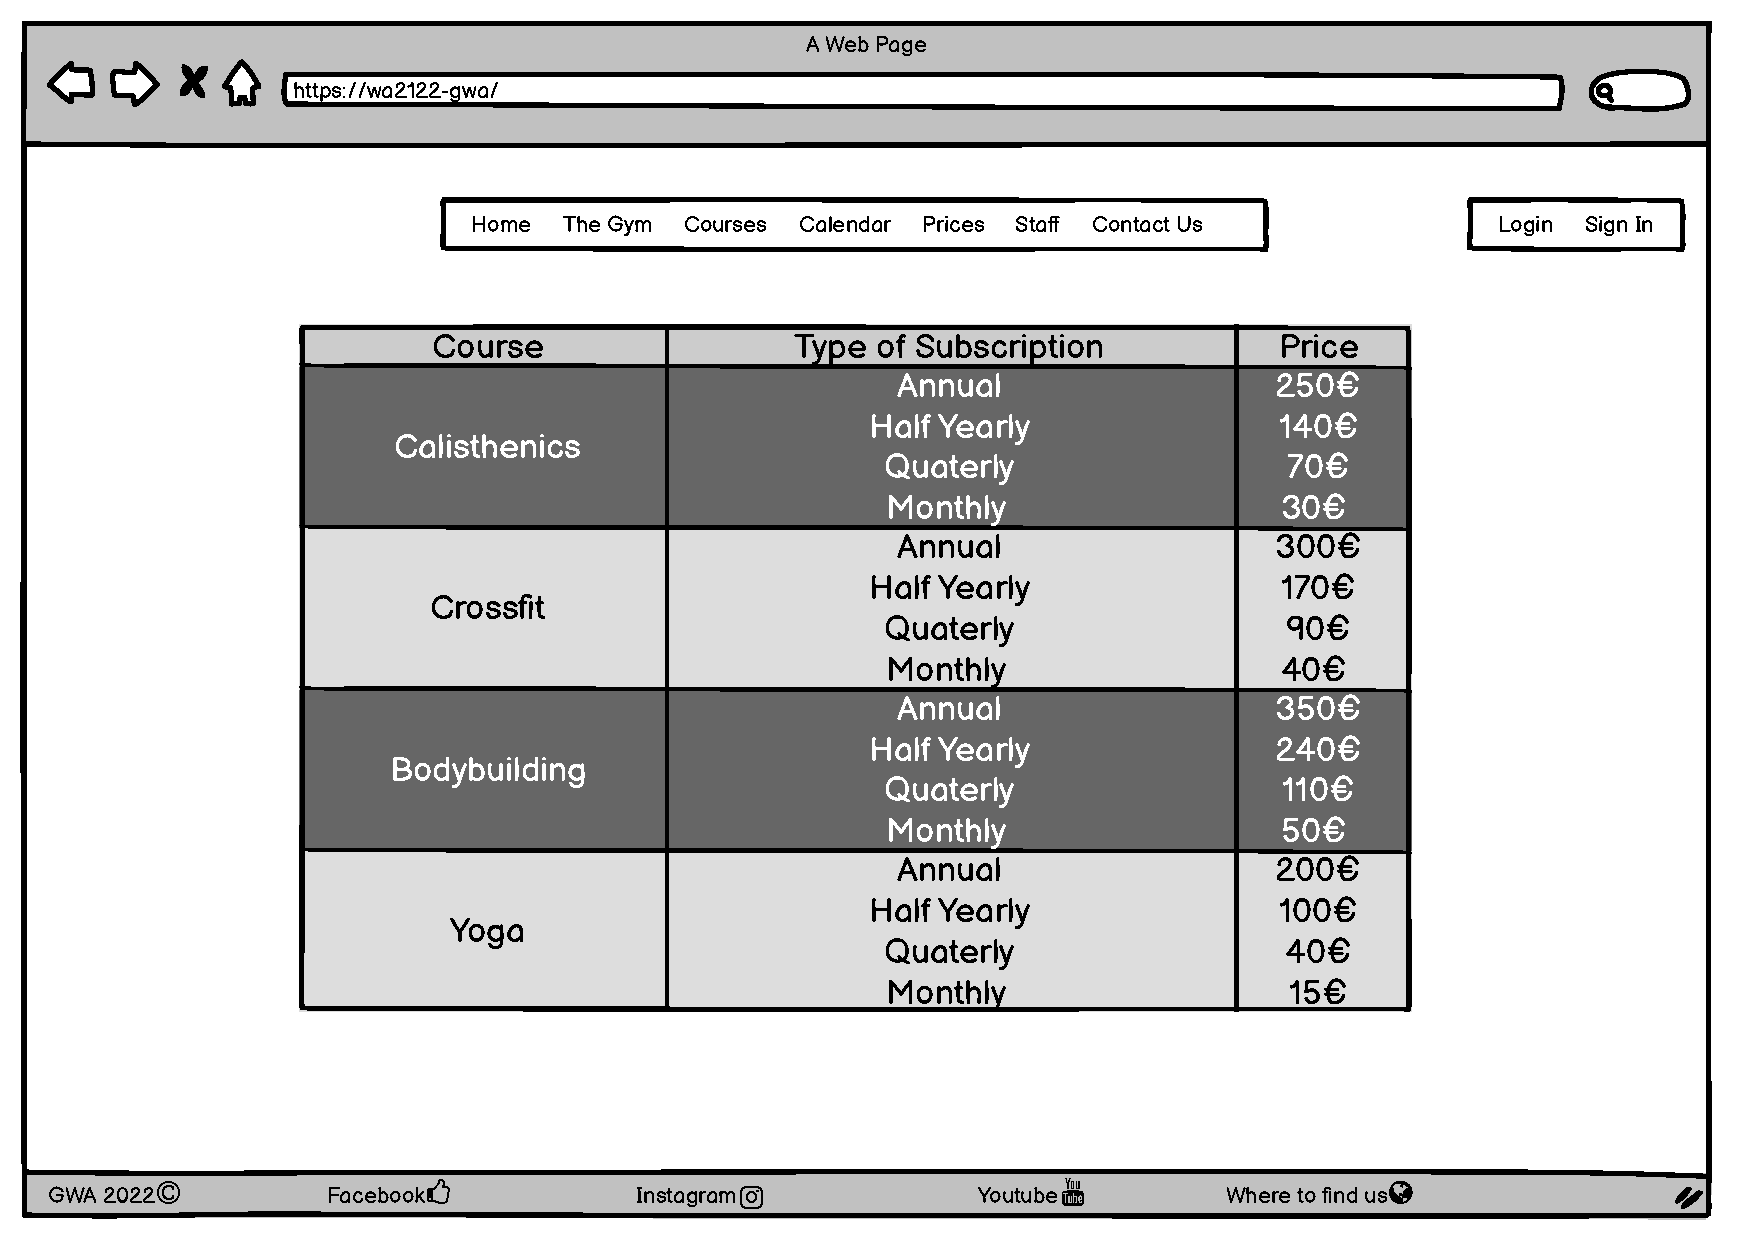
\includegraphics[width=\columnwidth]{InterfaceMockup/Prices/prices_page.pdf}

\subsubsection{Staff}
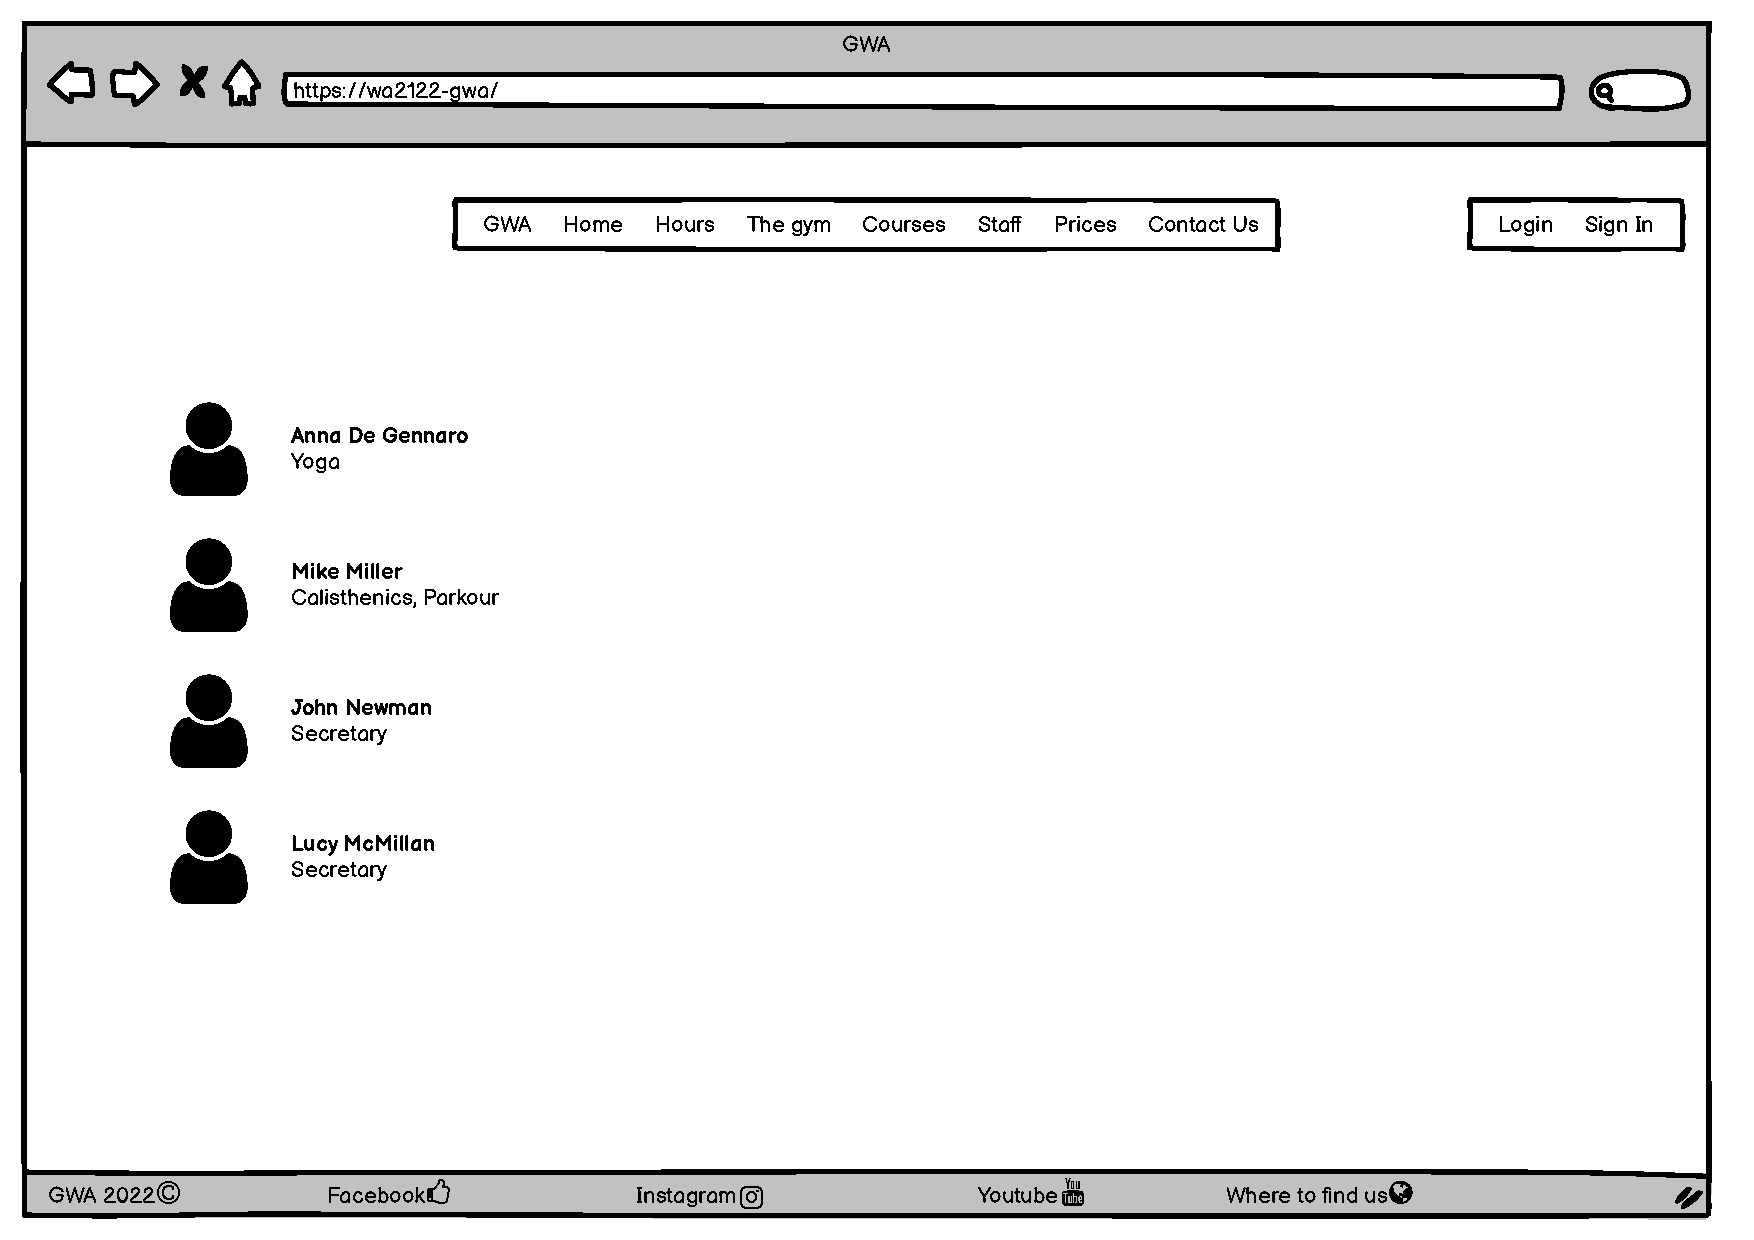
\includegraphics[width=\columnwidth]{InterfaceMockup/staff.pdf}

\subsubsection{Contact Us}
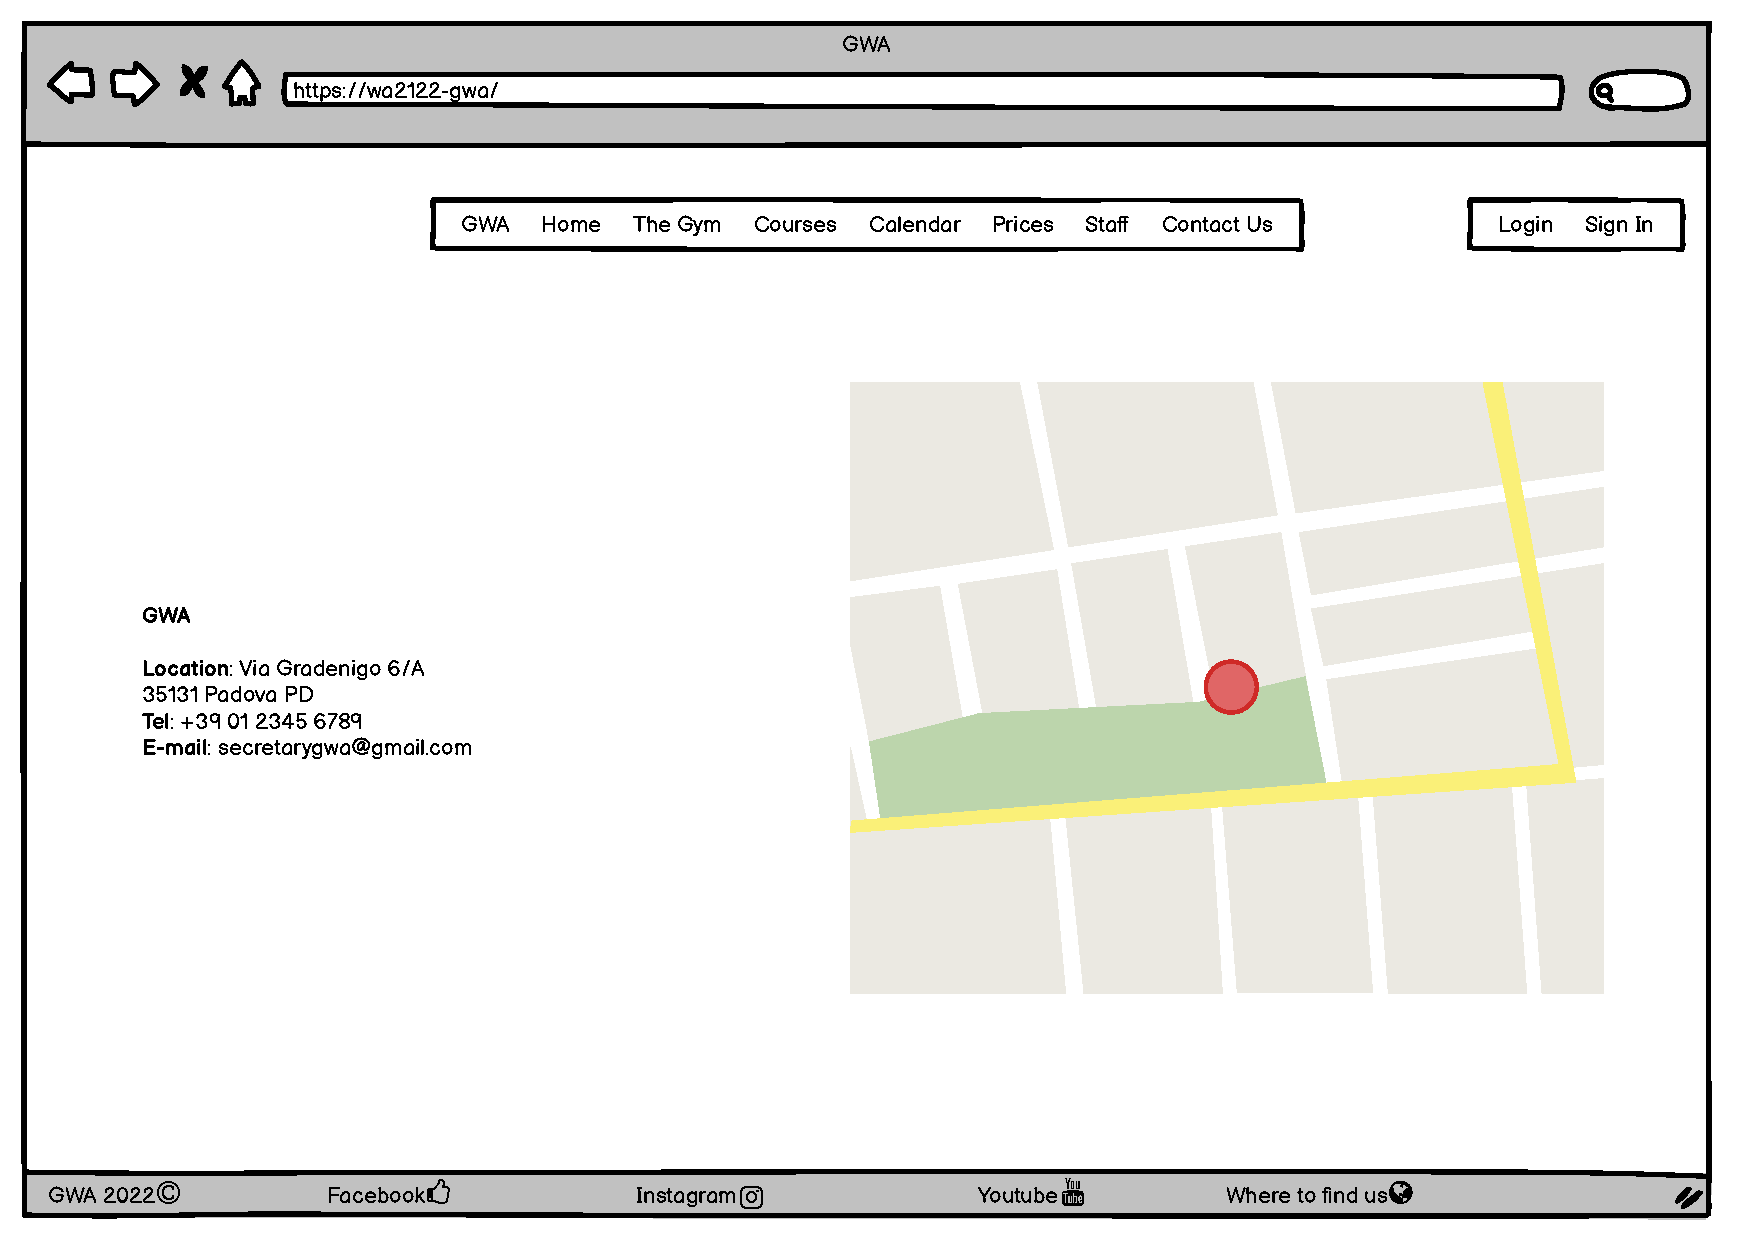
\includegraphics[width=\columnwidth]{InterfaceMockup/contact_us.pdf}

\subsubsection{Login}
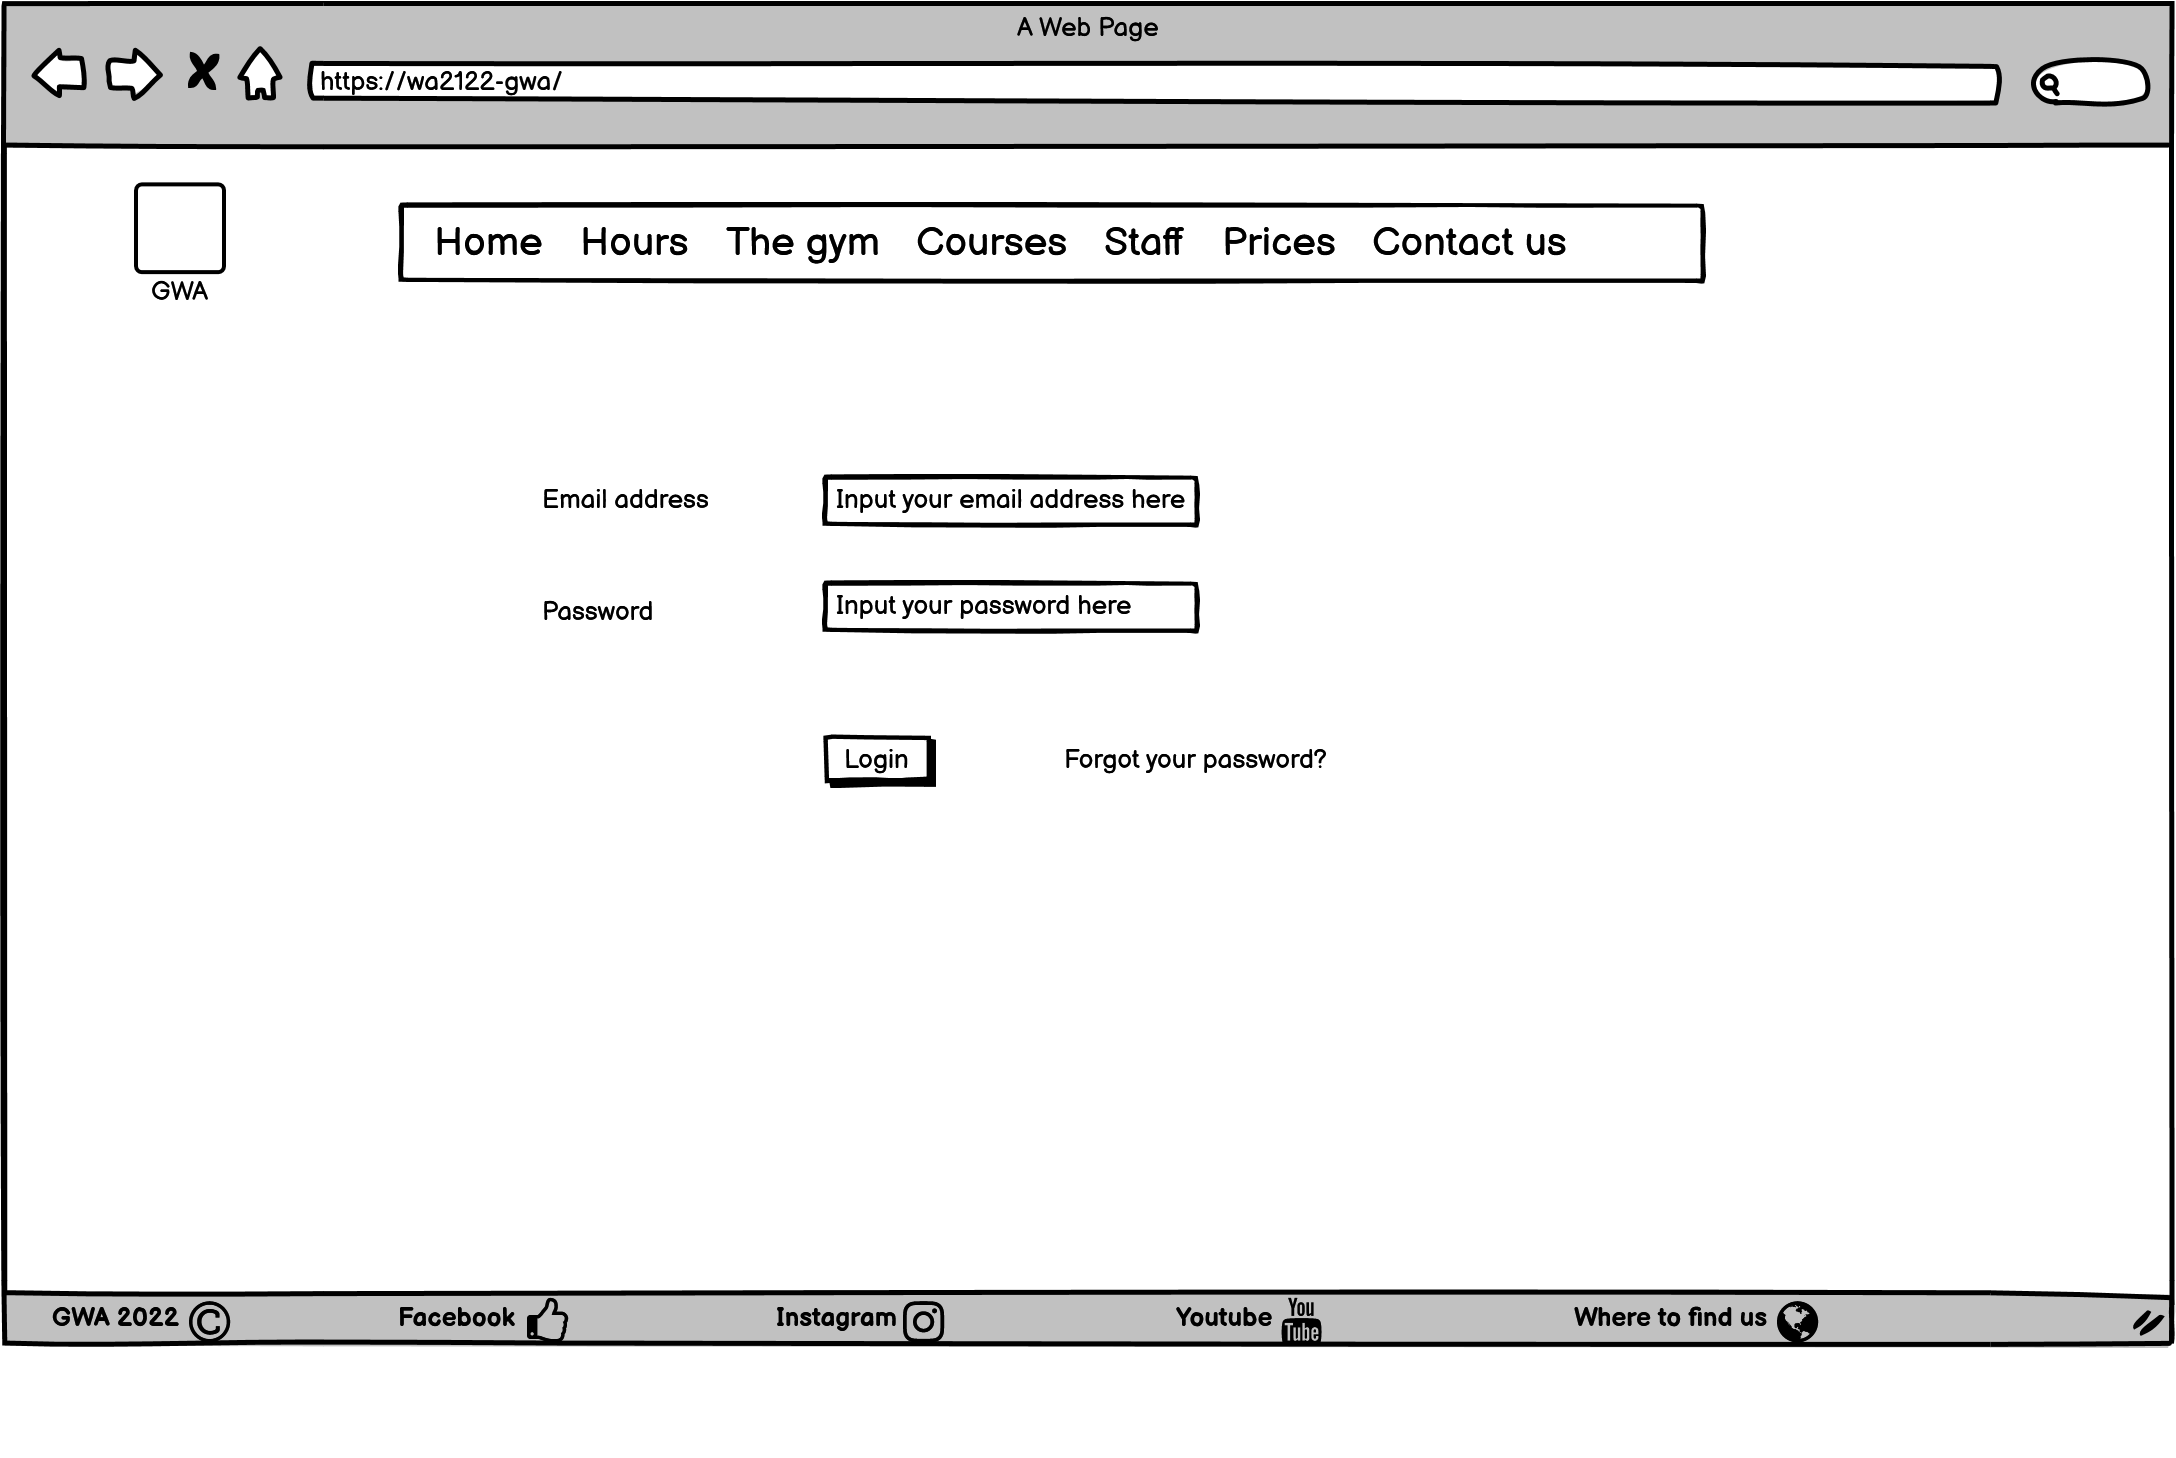
\includegraphics[width=\columnwidth]{InterfaceMockup/Login/Login.png}

\subsubsection{Register}
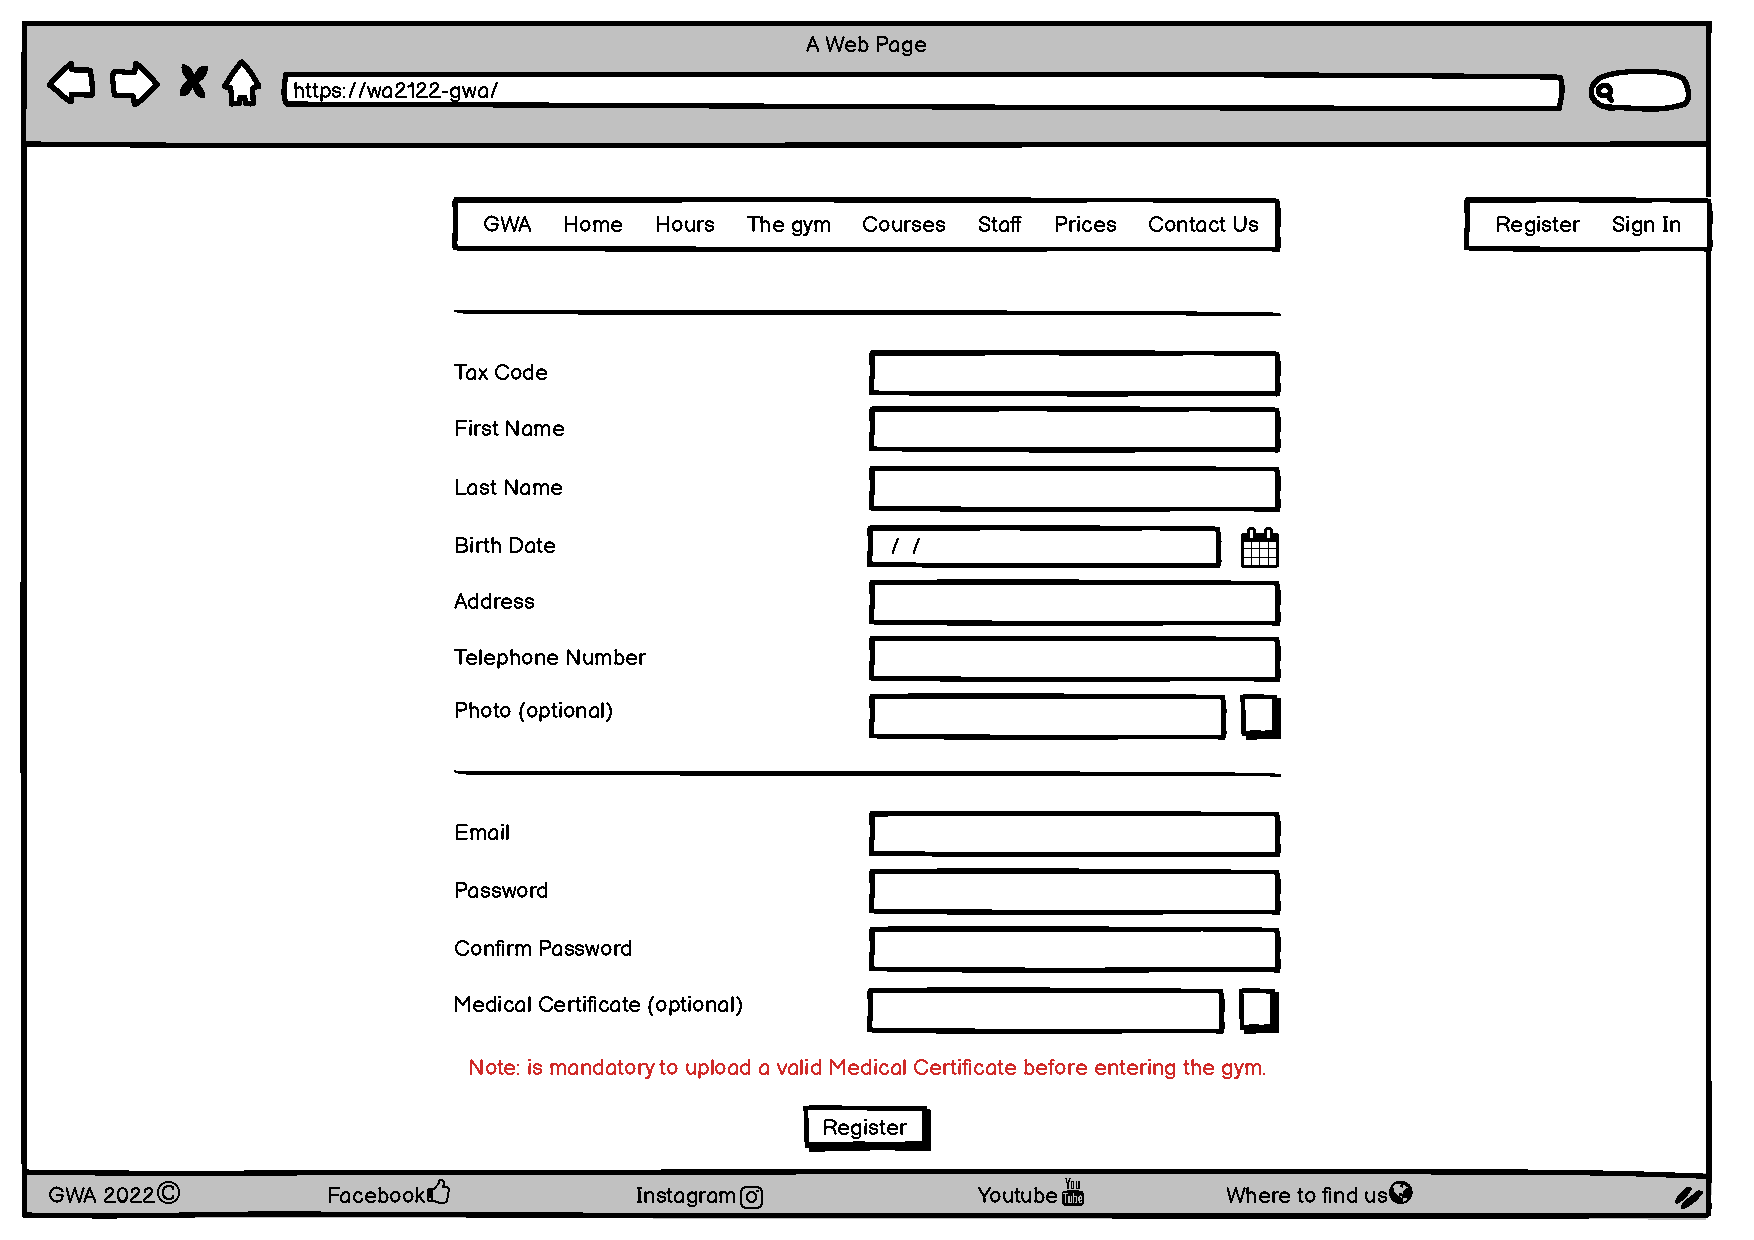
\includegraphics[width=\columnwidth]{InterfaceMockup/register.pdf}

\subsubsection{Trainee}
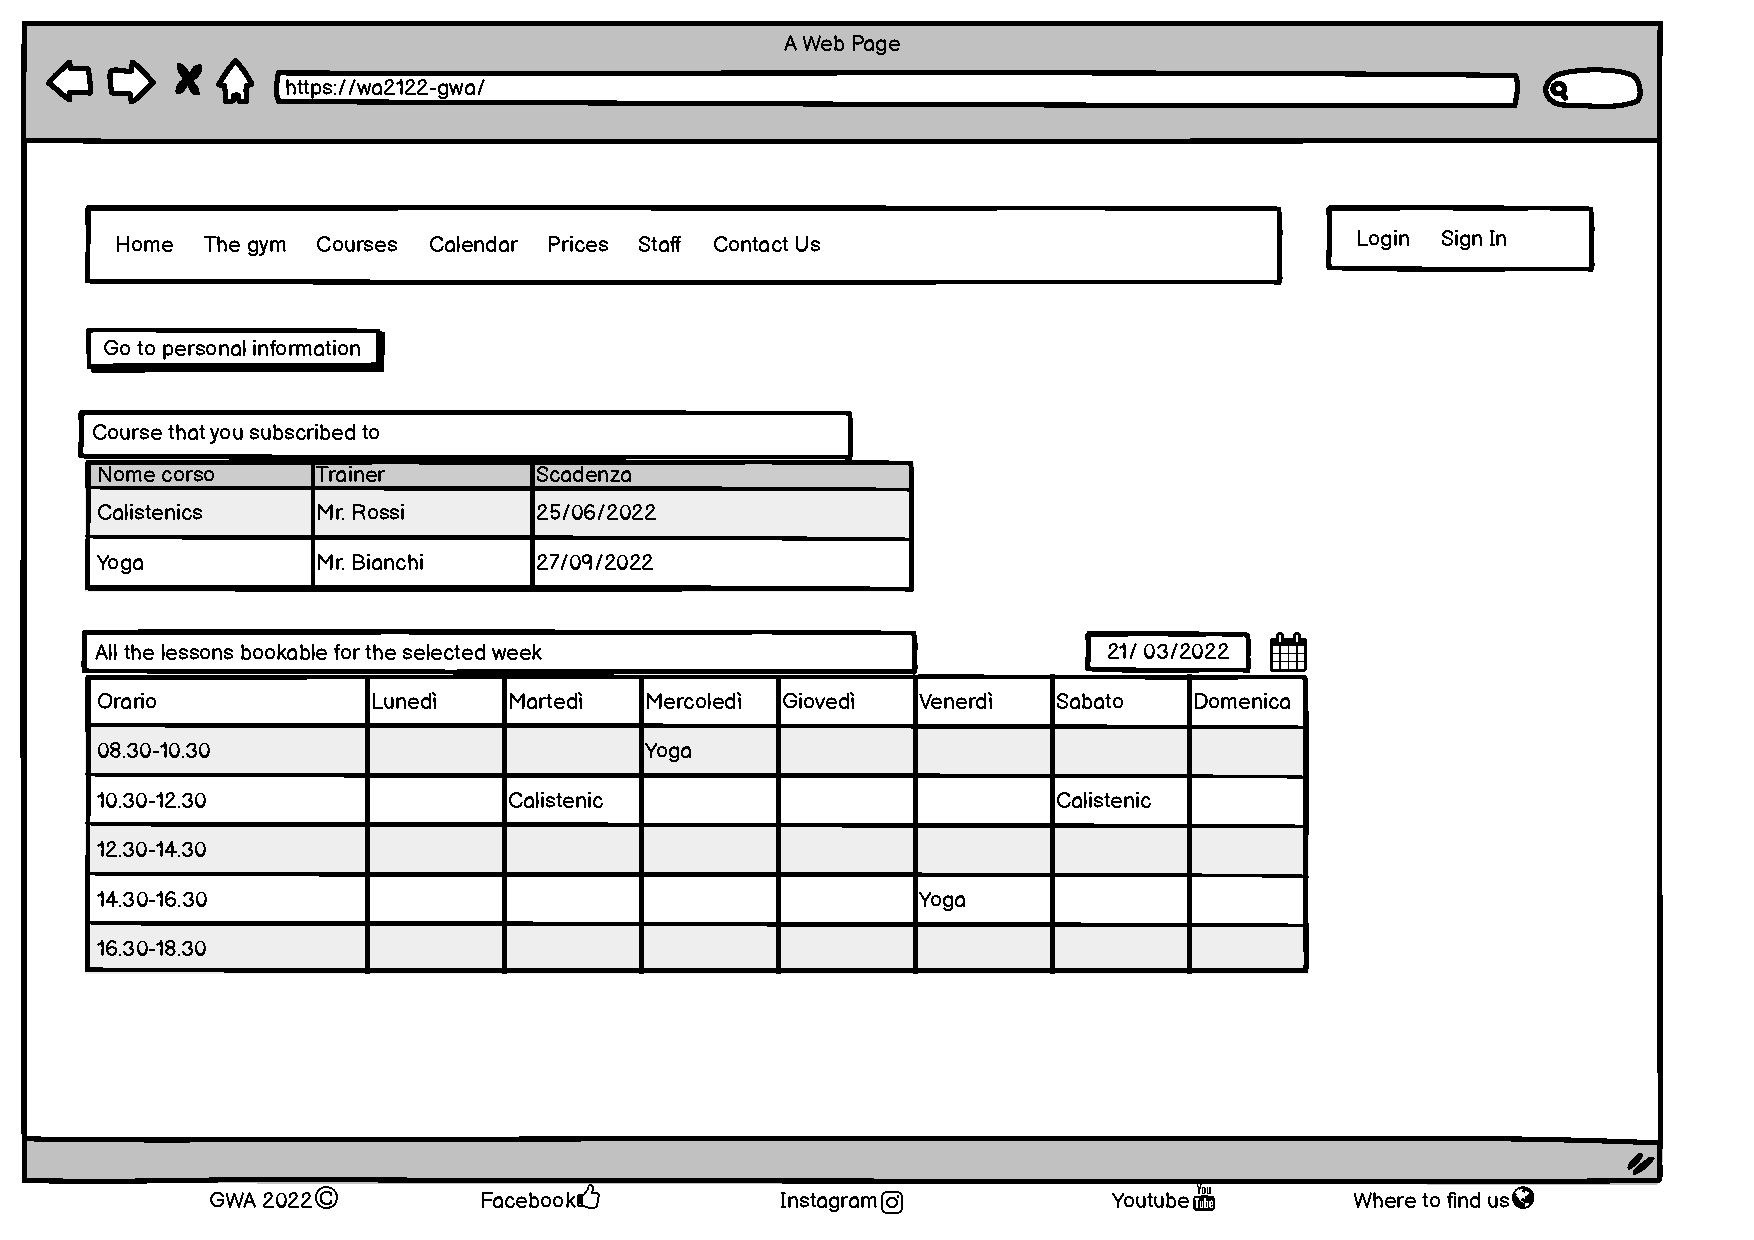
\includegraphics[width=\columnwidth]{InterfaceMockup/Trainee.pdf}

\subsubsection{Trainer}
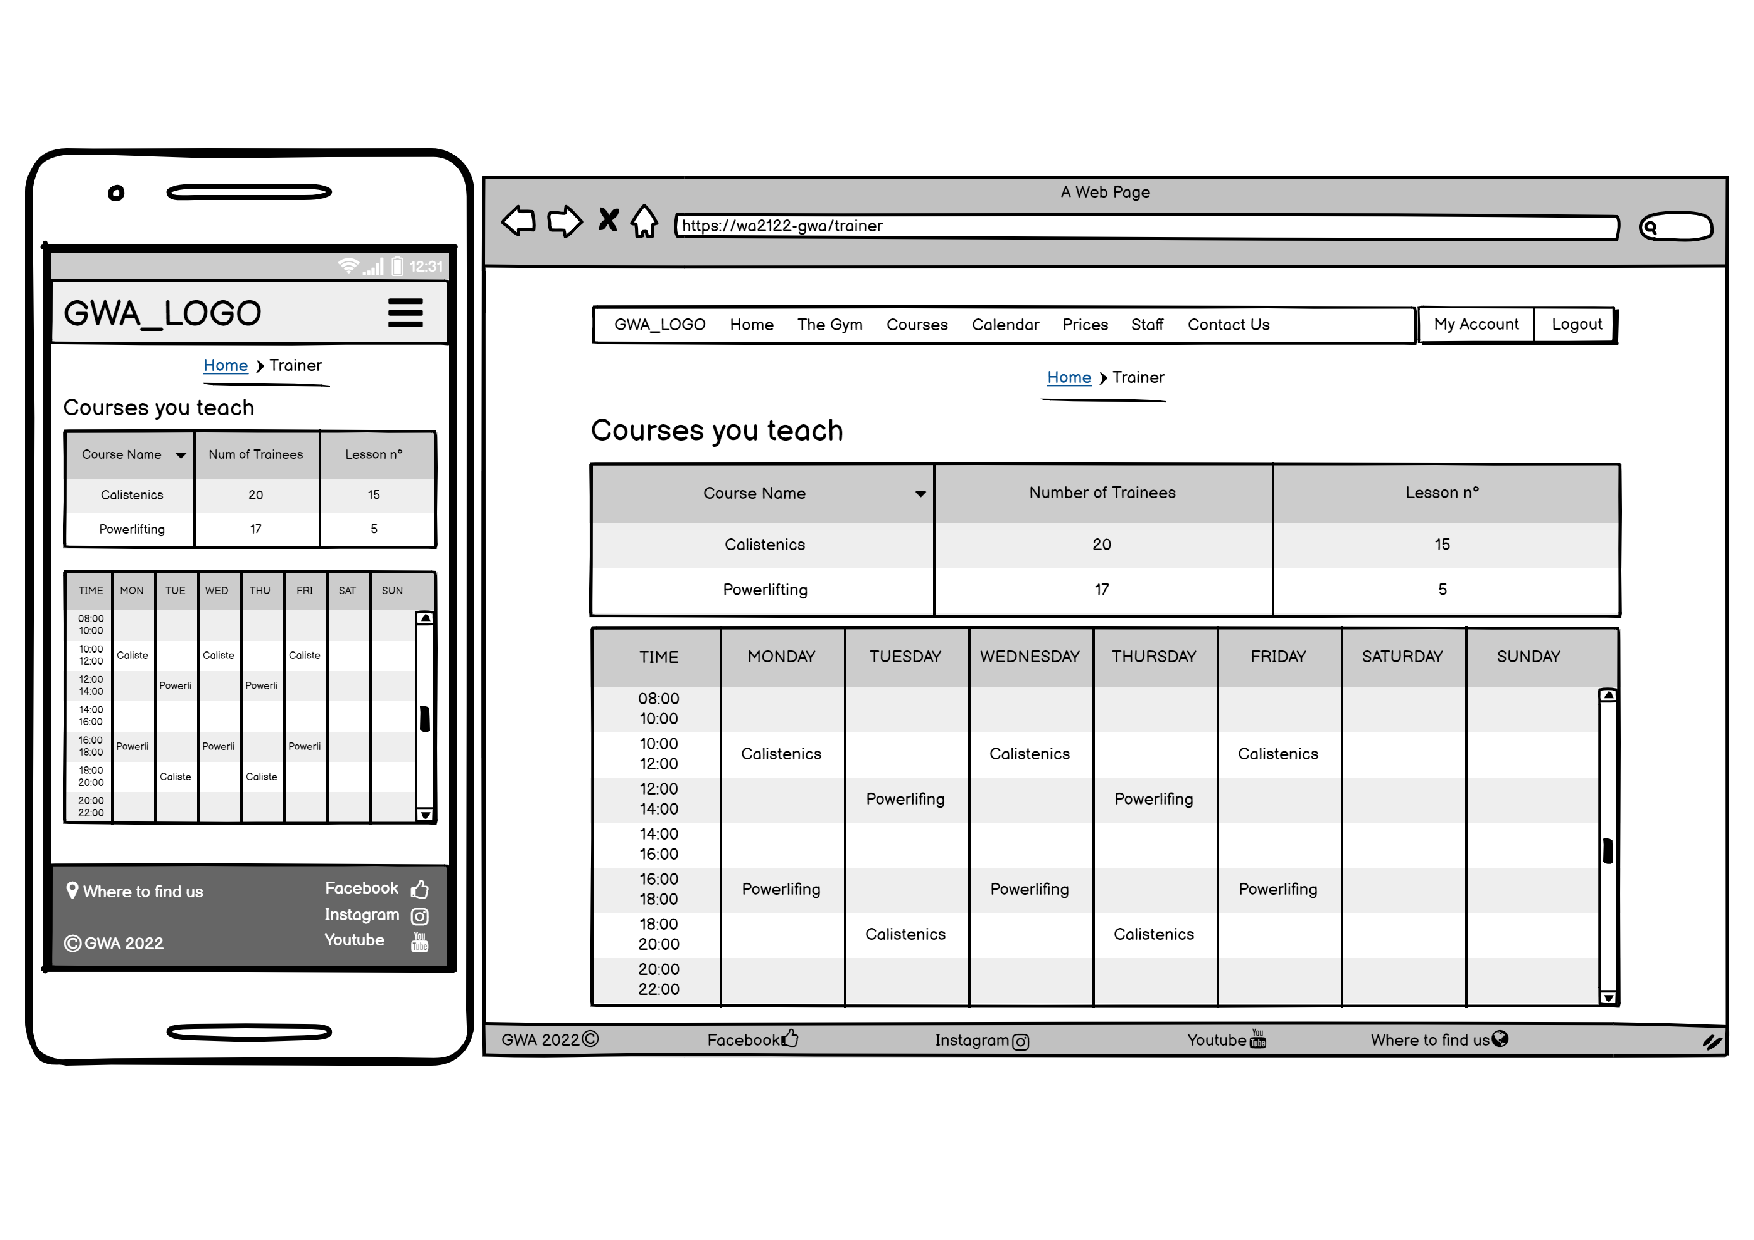
\includegraphics[width=\columnwidth]{InterfaceMockup/Trainer/Trainer.pdf}

\subsubsection{Secretary}

